\subsection{Graphs of Trigonometric Functions}
The graph of the functions $\sin x$ and $\cos x$ can be visually represented as:

$$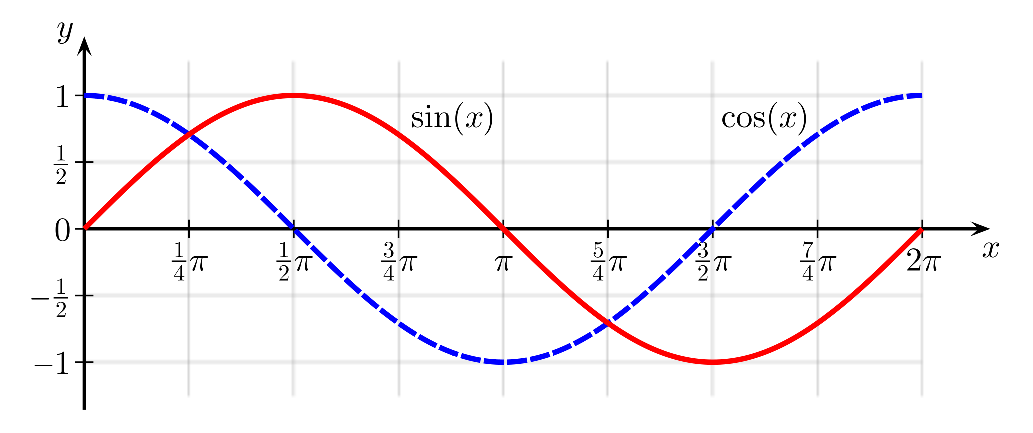
\includegraphics[width=4.0in]{images/sine-cosine}$$

Both $\sin x$ and $\cos x$ have domain $(-\infty,\infty)$ and range $[-1,1]$.
That is,
$$-1\leq\sin x\leq 1\qquad -1\leq\cos x\leq 1.$$
The zeros of $\sin x$ occur at the integer multiples of $\pi$, that is, $\sin x=0$ whenever $x=n\pi$, where $n$ is an integer.
Similarly, $\cos x=0$ whenever $x=\pi/2+n\pi$, where $n$ is an integer.

The six basic trigonometric functions can be visually represented as:

$$\includegraphics[width=7in]{images/trig-functions-new}$$

Both tangent and cotangent have range $(-\infty,\infty)$, whereas cosecant and secant have range $(-\infty,-1]\cup[1,\infty)$.
Each of these functions is periodic. Tangent and cotangent have period $\pi$, whereas sine, cosine, cosecant and secant have period $2\pi$.